\chapter{Implementasi}
\section{Lingkungan Implementasi}
Sesudah menyelesaikan proses analisis, proses yang dilakukan pada tahap selanjutnya adalah perancanagan program dimana semua dijalankan secara otomatis pada tahap mencari dan mendownload.


\subsection{Menggunakan Selenium}
    Pada tahap ini bagaimana menjalannkan progran otomatis dengan web testing menggunakan Python dan menggunkan IDE Spyder. Disini Program Menjalankan Printah otomatis Membuka,mengambil url sampai muncul nya akses download secara otomatis, dengan codingan yaitu: :

\begin{enumerate}
    \item search=('tuf') :
    merupakan variable yang menampung nilai string dimana Tuf adalah judul video yang dicari
    \item youtube = webdriver.Firefox() :
    merupakan variable yang akan memanggil webdriver Firefox
    \item youtube.get('https://www.youtube.com/') :
    variable yang berisikan alamat url dari youtube 
    \item youtube.get('https://www.youtube.com/results?search-query= '+ search) :
    varible yang akan memanggil youtube serta penambahan variable dari search. fungsi dari search inilah yang memberikan judul dari video yang akan di cari
    \item youtube.get('https://en.savefrom.net/') :
    variable yang memanggil savefrom.net melalui url
    \item youtube.find\_element\_by\_id('sf-url').send\_keys('https://www.youtube.com/watch
    ?v=wyrbTx85gWM') :
    codingan ini berfungsi sebagai media tempat paste url dari youtube dan membeberikan url video
    \item youtube.find\_element|\_by\_xpath('//*[@id="sf-submit"]').click() :
    codingan ini berfungsi memunculjkan tampilan download yang ada pada savefrom.net.
    \item sleep(3) : memberikan jeda waktu 3 detik untuk menampilakan tombol download 
    \item youtube.find\_element\_by\_xpath('/html/body/div/div[1]/div[3]/div[4]/div/div[1]
    /div[2]/div[2]/div[1]/a').click() : codingan yang berfungsi  untuk menekan tombol download pada savefrom.net secara otomatis.
\end{enumerate}

\subsection{Cara pengambilan Element pada Web }
    Pada Tahapan ini akan diberitahu cara mengambil element sebagi berikut:

\begin{enumerate}
    \item Kita ambil contoh website tersebut adalah savefrom.net. Kita akan Inspect kode Program.
\begin{figure}[!htbp]
    \centering
    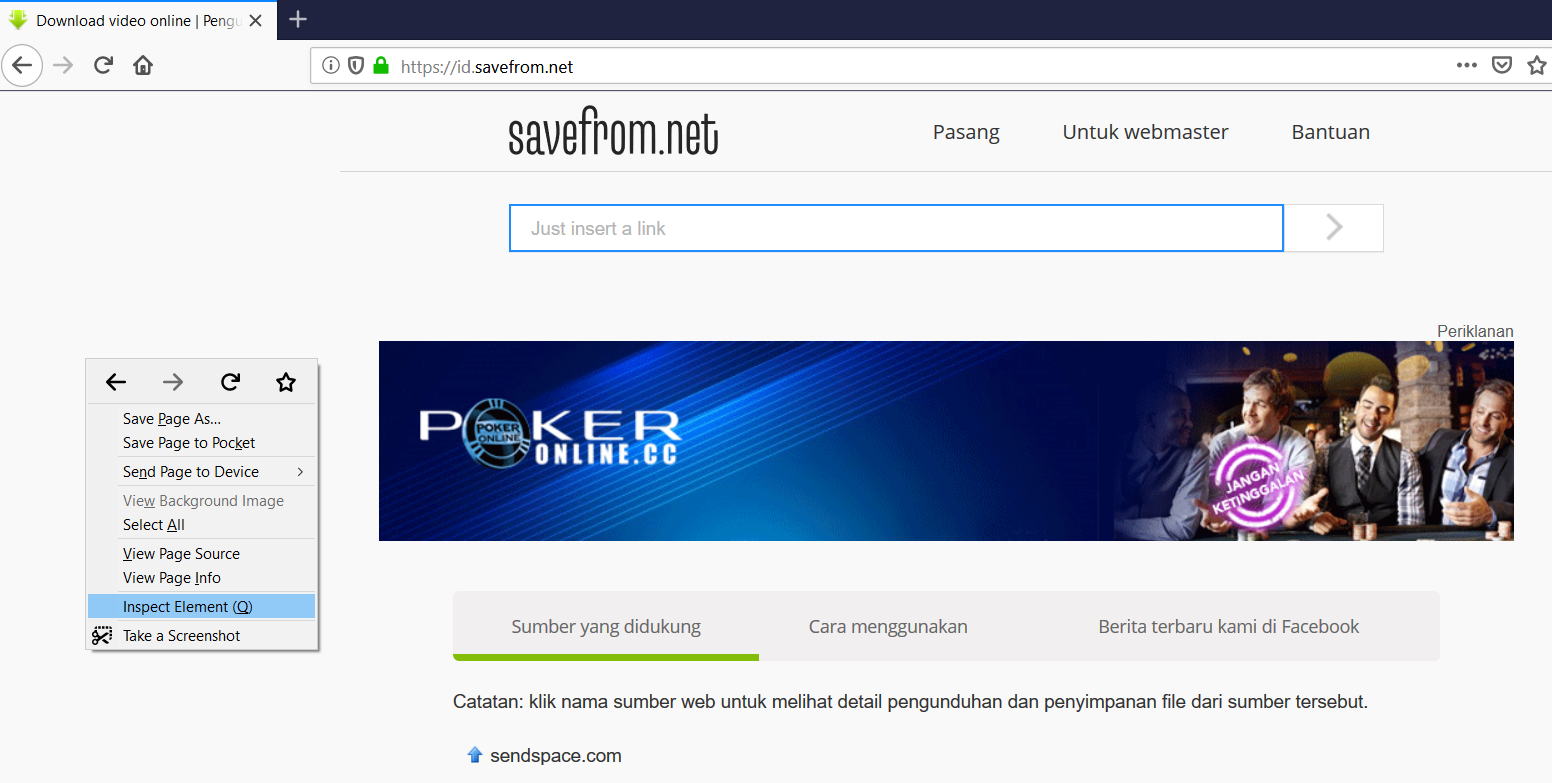
\includegraphics[scale=0.3]{figure/inspect.png}
    \label{gambar 1}
\end{figure}
    \item Kemudian ketika menekan inspect maka akan muncul hasil dari inspect code program, kemudian klik kanan, kemudian pada menu copy klik xpath.
\begin{figure}[!htbp]
    \centering
    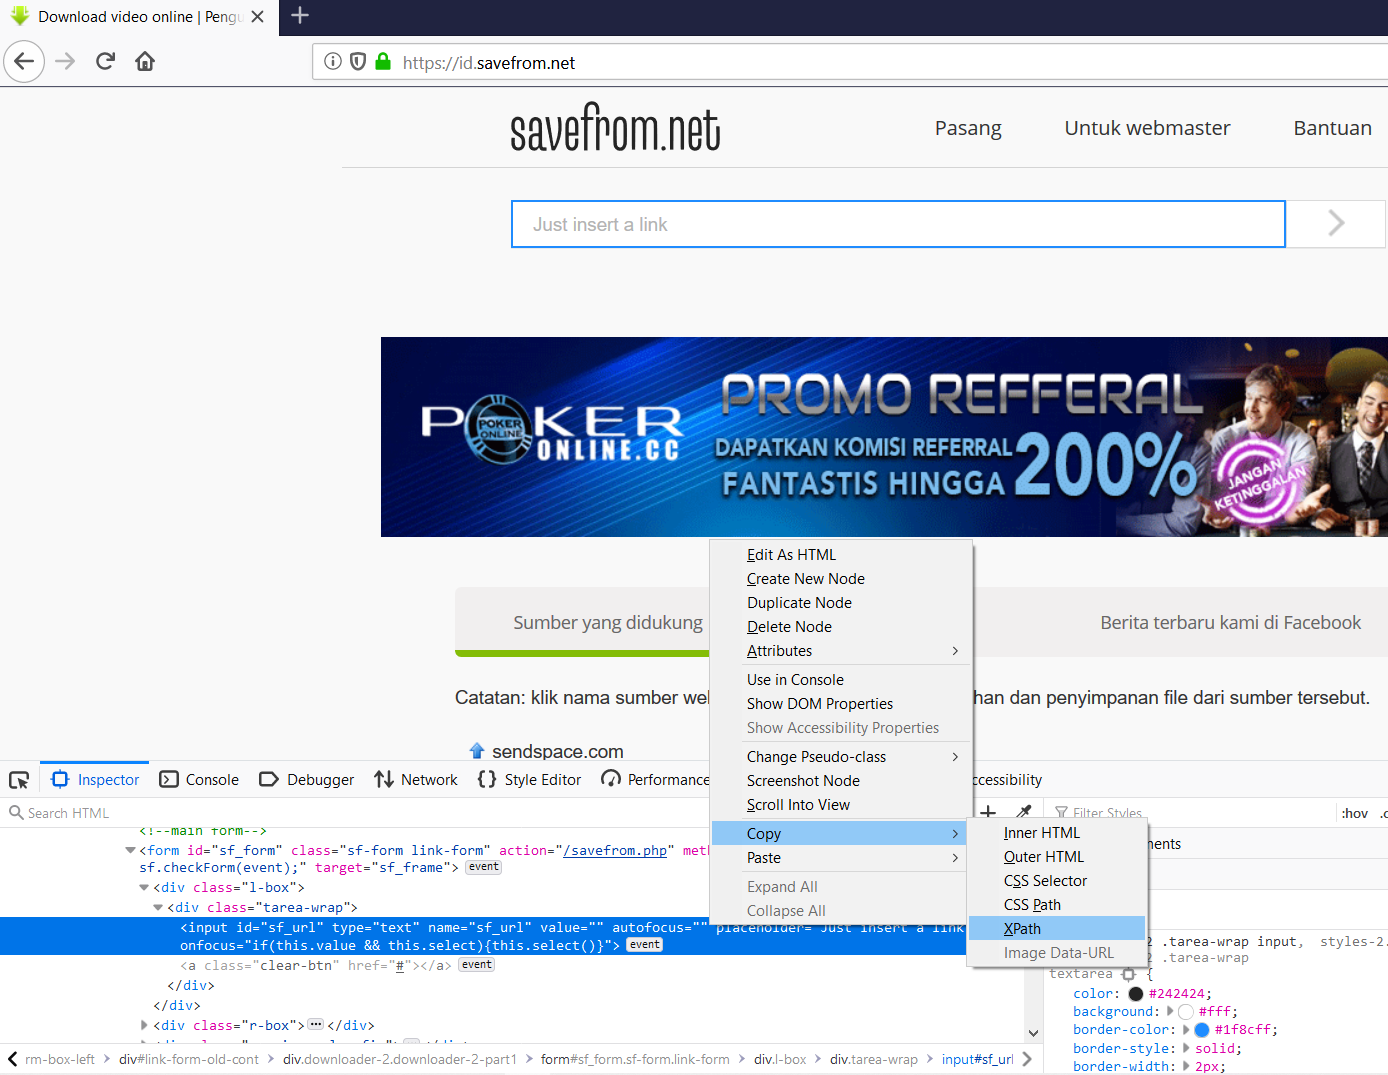
\includegraphics[scale=0.3]{figure/hasil1.png}
    \label{gambar 4}
\end{figure}
\end{enumerate}
  
\section{Pengujian dan Hasil Pengujian}
\subsection{Pengujian}
Berikut ini ada beberapa tahapan pengujian jalannya pengoperasian download secara otomotis 

\begin{enumerate}
    \item Kita menggunakan find\_element sebagai Pemberikan text secara otomatis. Saat  Di run hasil pada menu search pada youtube tidak muncul text yang telah ditentukan. Dan pada Spyder {(unknown variant search)}
\begin{figure}[!htbp]
    \centering
    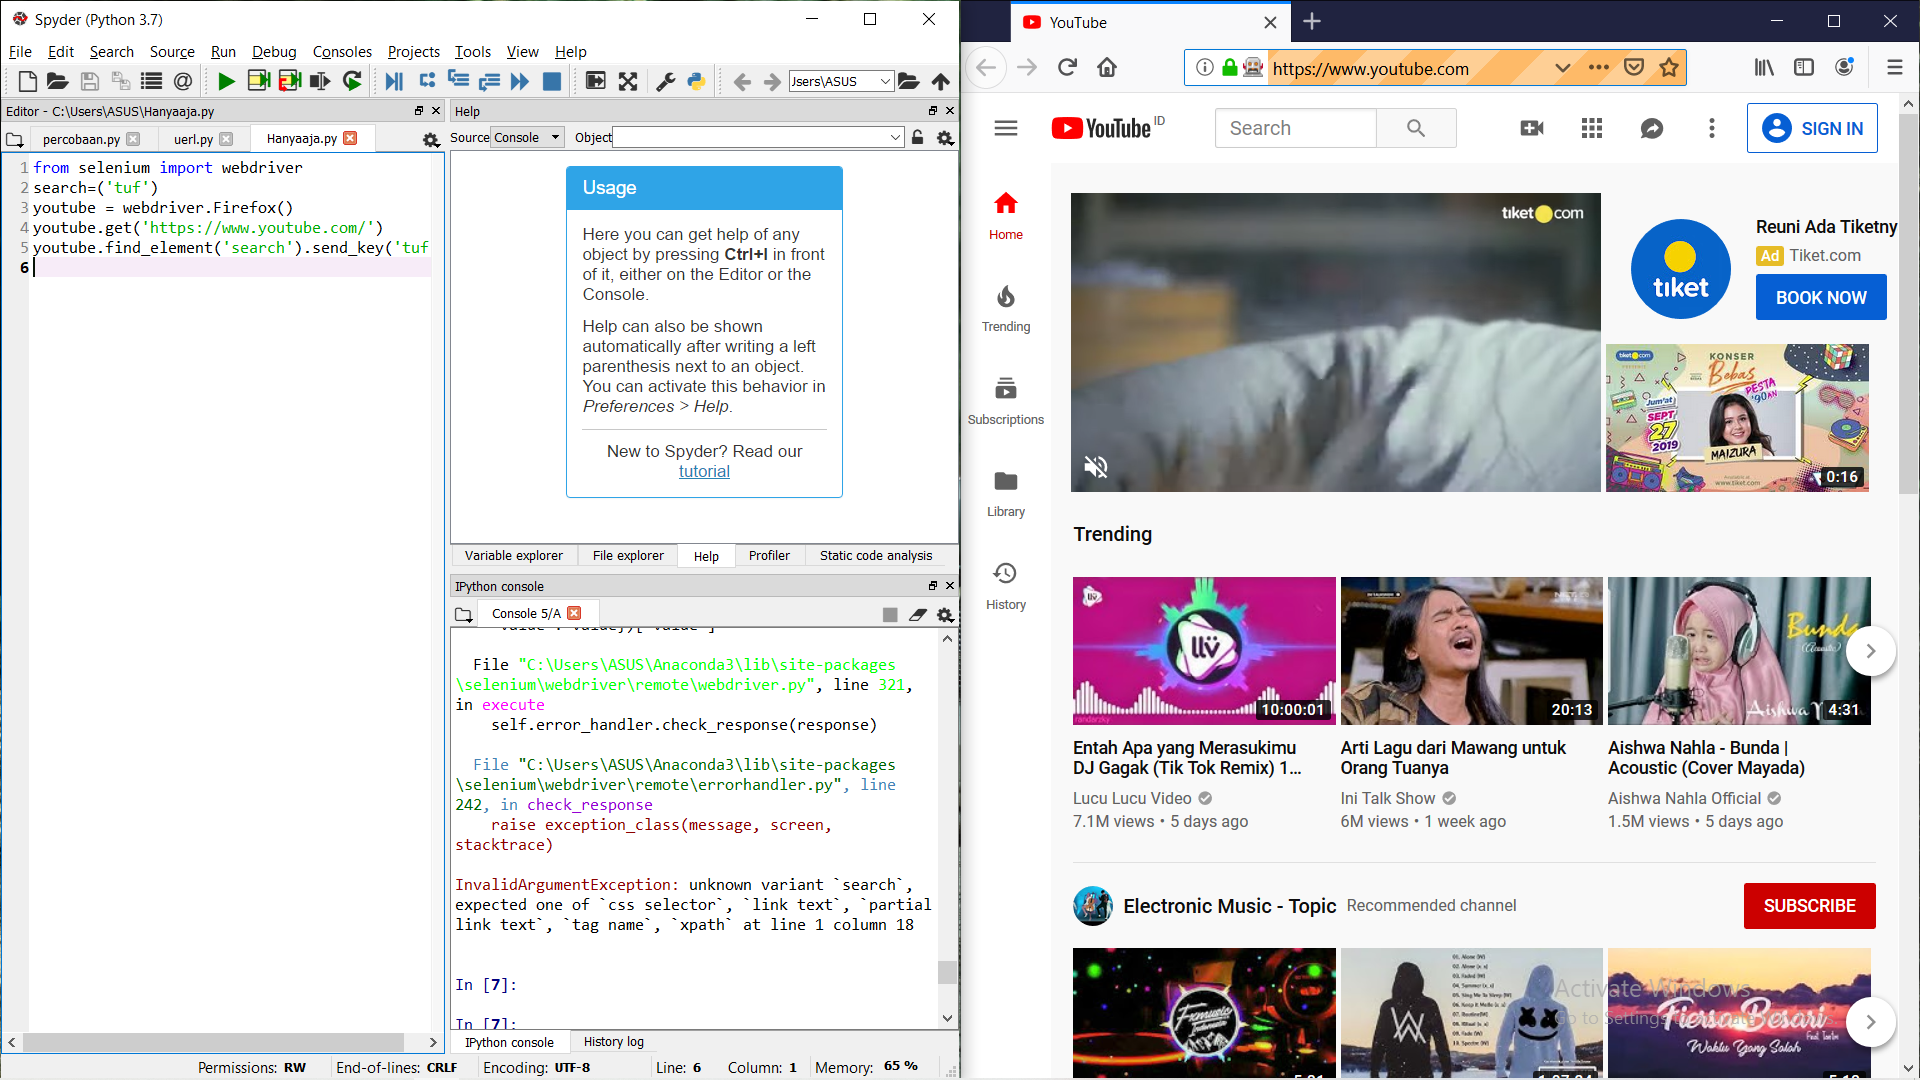
\includegraphics[scale=0.3]{figure/hasilTes/1.png}
    \label{gambar 1}
\end{figure}
\vspace{10cm}
    \item Kita menggunakan find\_element\_by\_class\_name sebagai Pemberikan text secara otomatis. Saat  Di run hasil pada menu search pada youtube tidak muncul text yang telah ditentukan. Dan pada Spyder {(unknown variant search)}
\begin{figure}[!htbp]
    \centering
    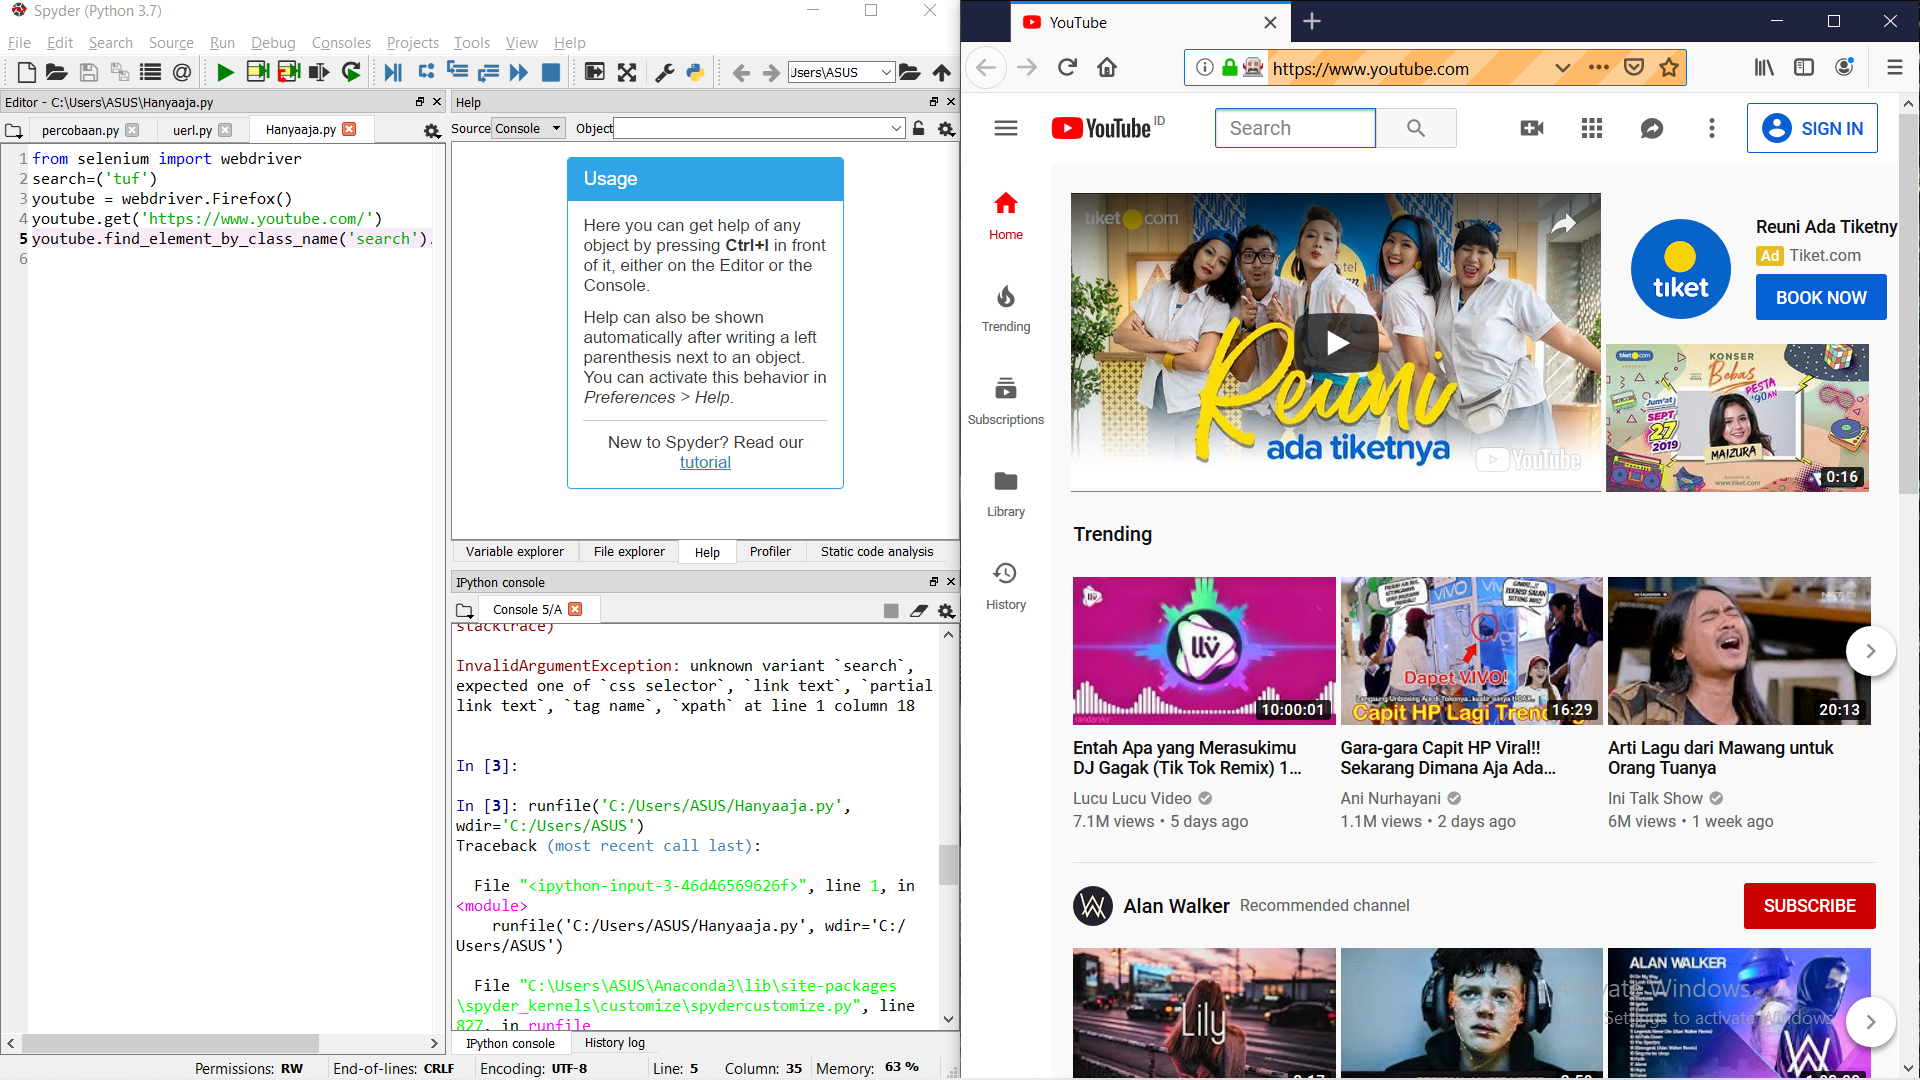
\includegraphics[scale=0.3]{figure/hasilTes/2.png}
    \label{gambar 1}
\end{figure}

     \item Kita menggunakan find\_element\_by\_id sebagai Pemberikan text secara otomatis. Saat  Di run hasil pada menu search pada youtube tidak muncul text yang telah ditentukan. Dan pada Spyder {(unable to locate search element)}
\begin{figure}[!htbp]
    \centering
    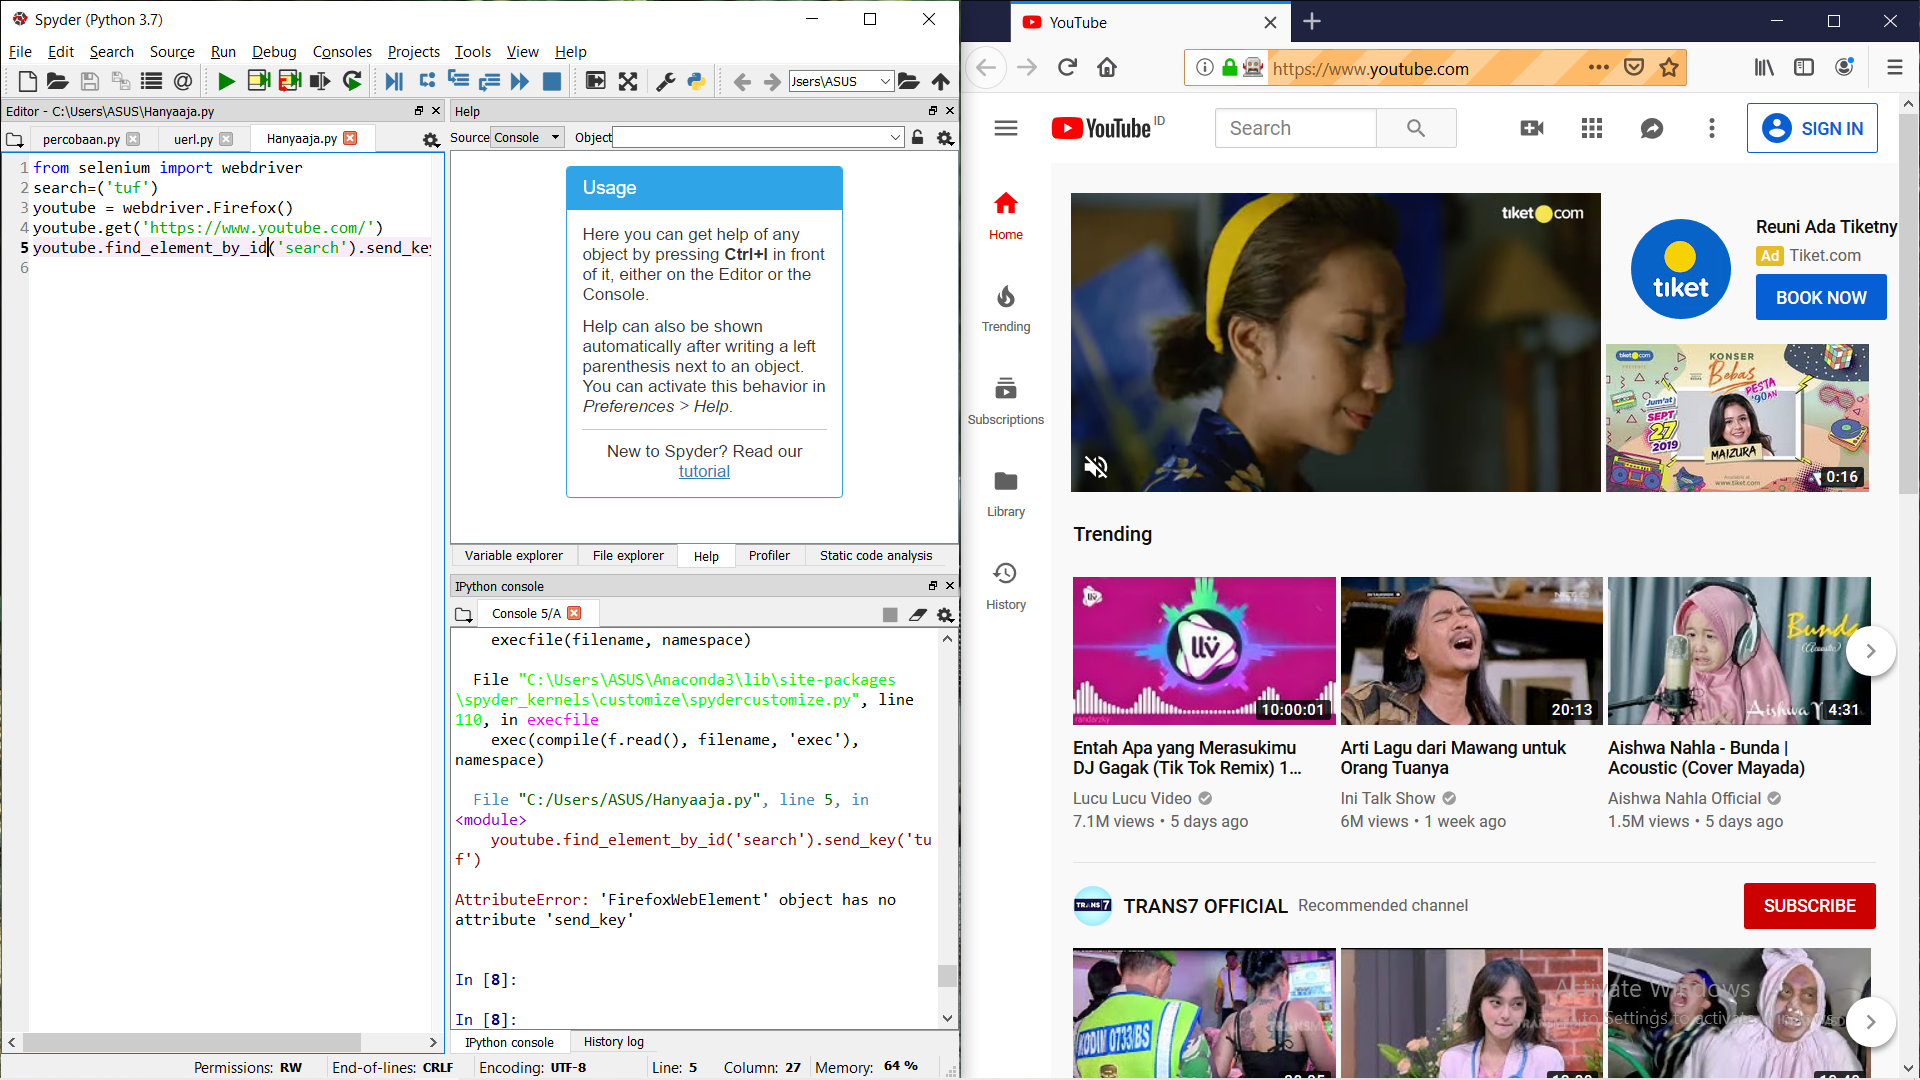
\includegraphics[scale=0.3]{figure/hasilTes/3.png}
    \label{gambar 1}
\end{figure}

    \item Kita menggunakan find\_element\_by\_link\_text sebagai Pemberikan text secara otomatis. Saat  Di run hasil pada menu search pada youtube tidak muncul text yang telah ditentukan. Dan pada Spyder {(unable to locate search element)}
\begin{figure}[!htbp]
    \centering
    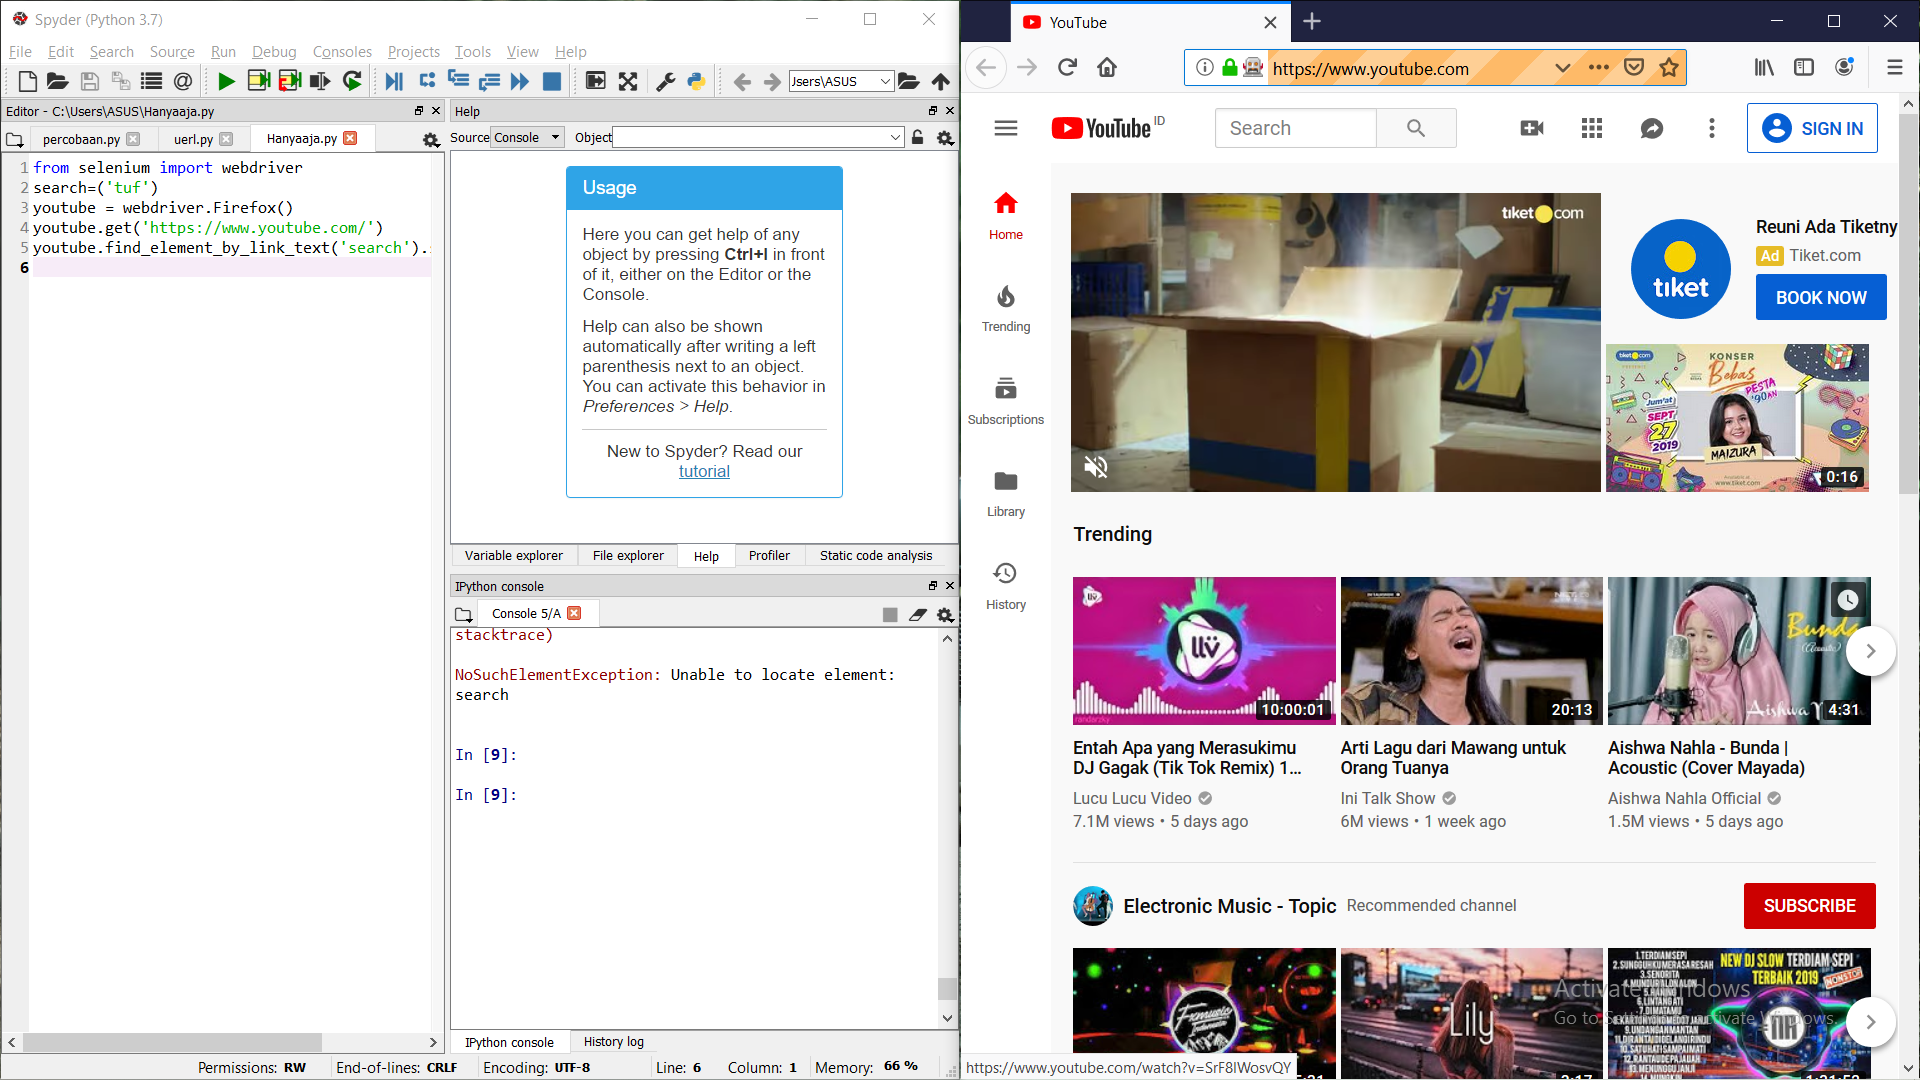
\includegraphics[scale=0.3]{figure/hasilTes/4.png}
    \label{gambar 1}
\end{figure}

    \item Kita menggunakan find\_element\_by\_name sebagai Pemberikan text secara otomatis. Saat  Di run hasil pada menu search pada youtube tidak muncul text yang telah ditentukan. Dan pada Spyder {(unable to locate name='search')}
\begin{figure}[!htbp]
    \centering
    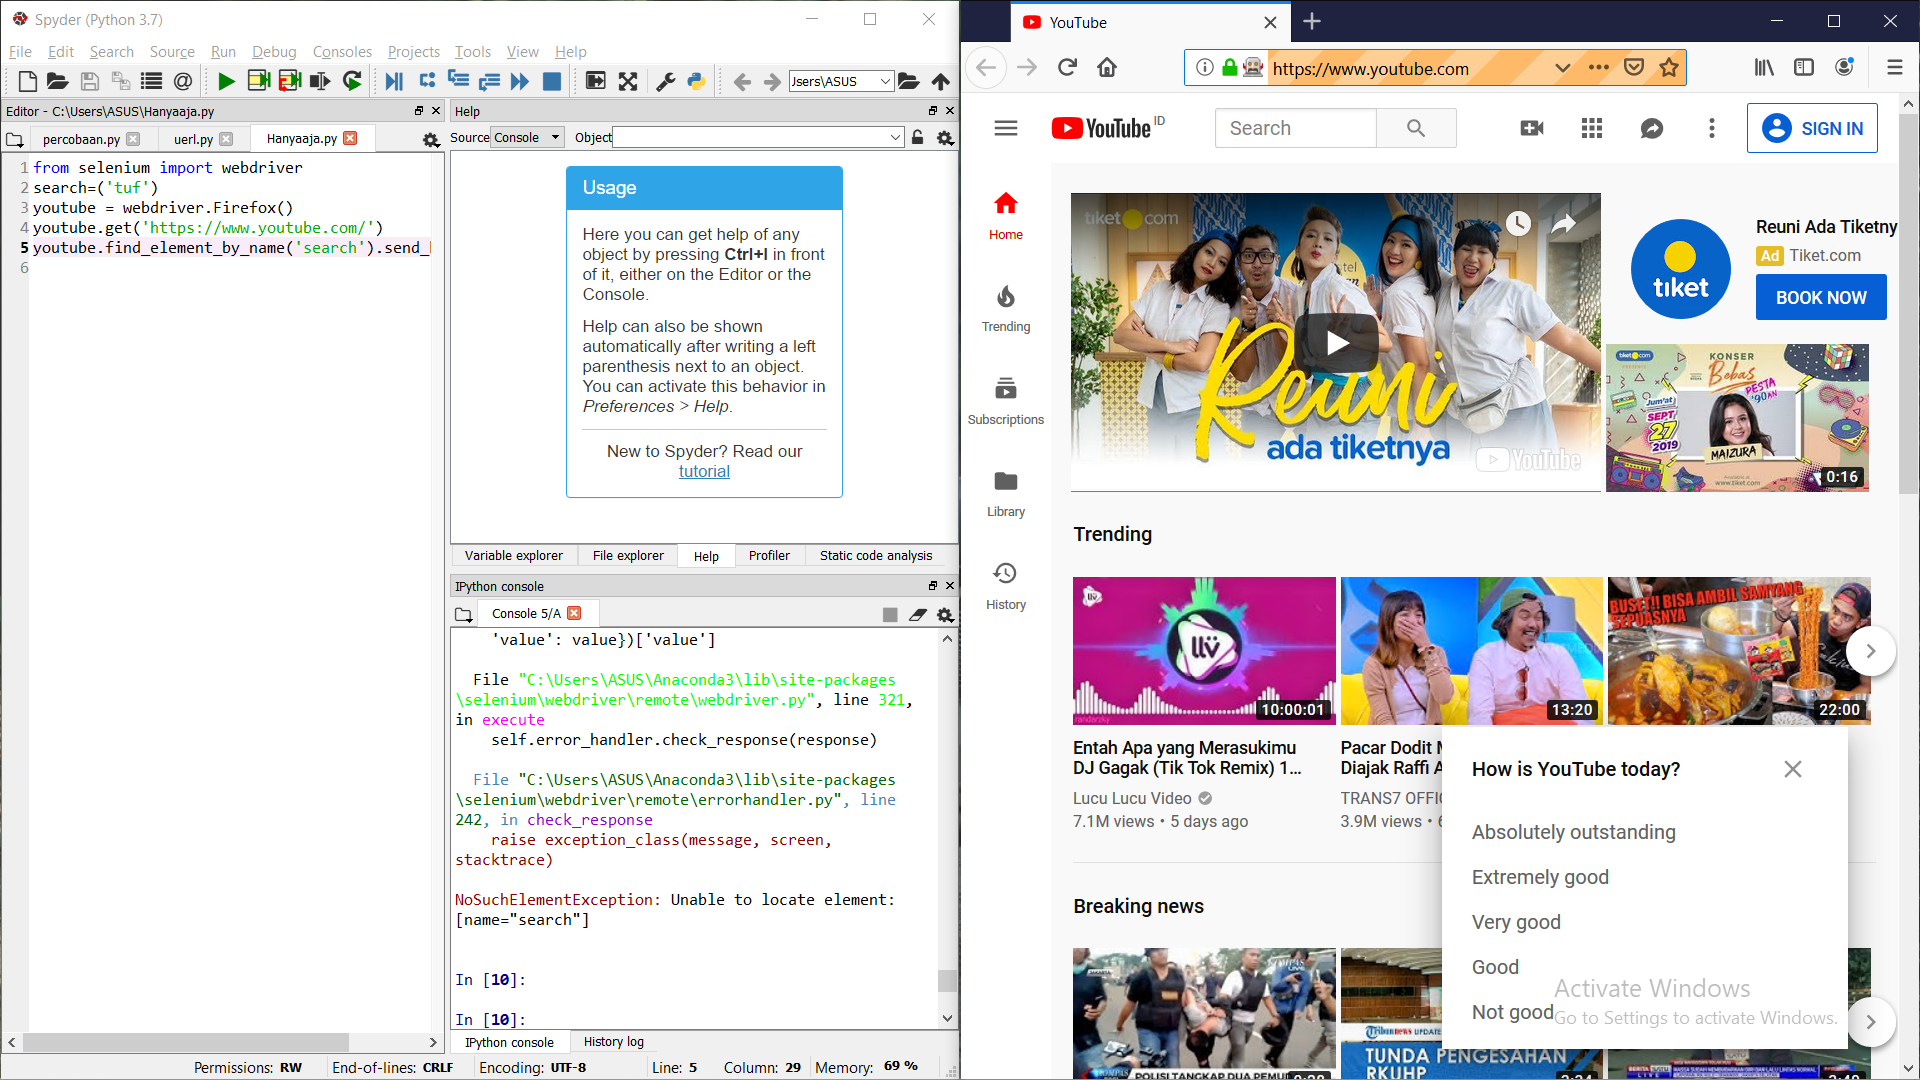
\includegraphics[scale=0.3]{figure/hasilTes/5.png}
    \label{gambar 1}
\end{figure}

    \item Kita menggunakan find\_element\_by\_partial\_link\_text sebagai Pemberikan text secara otomatis. Saat  Di run hasil pada menu search pada youtube tidak muncul text yang telah ditentukan. Dan pada Spyder {(unable to locate search element)}
\begin{figure}[!htbp]
    \centering
    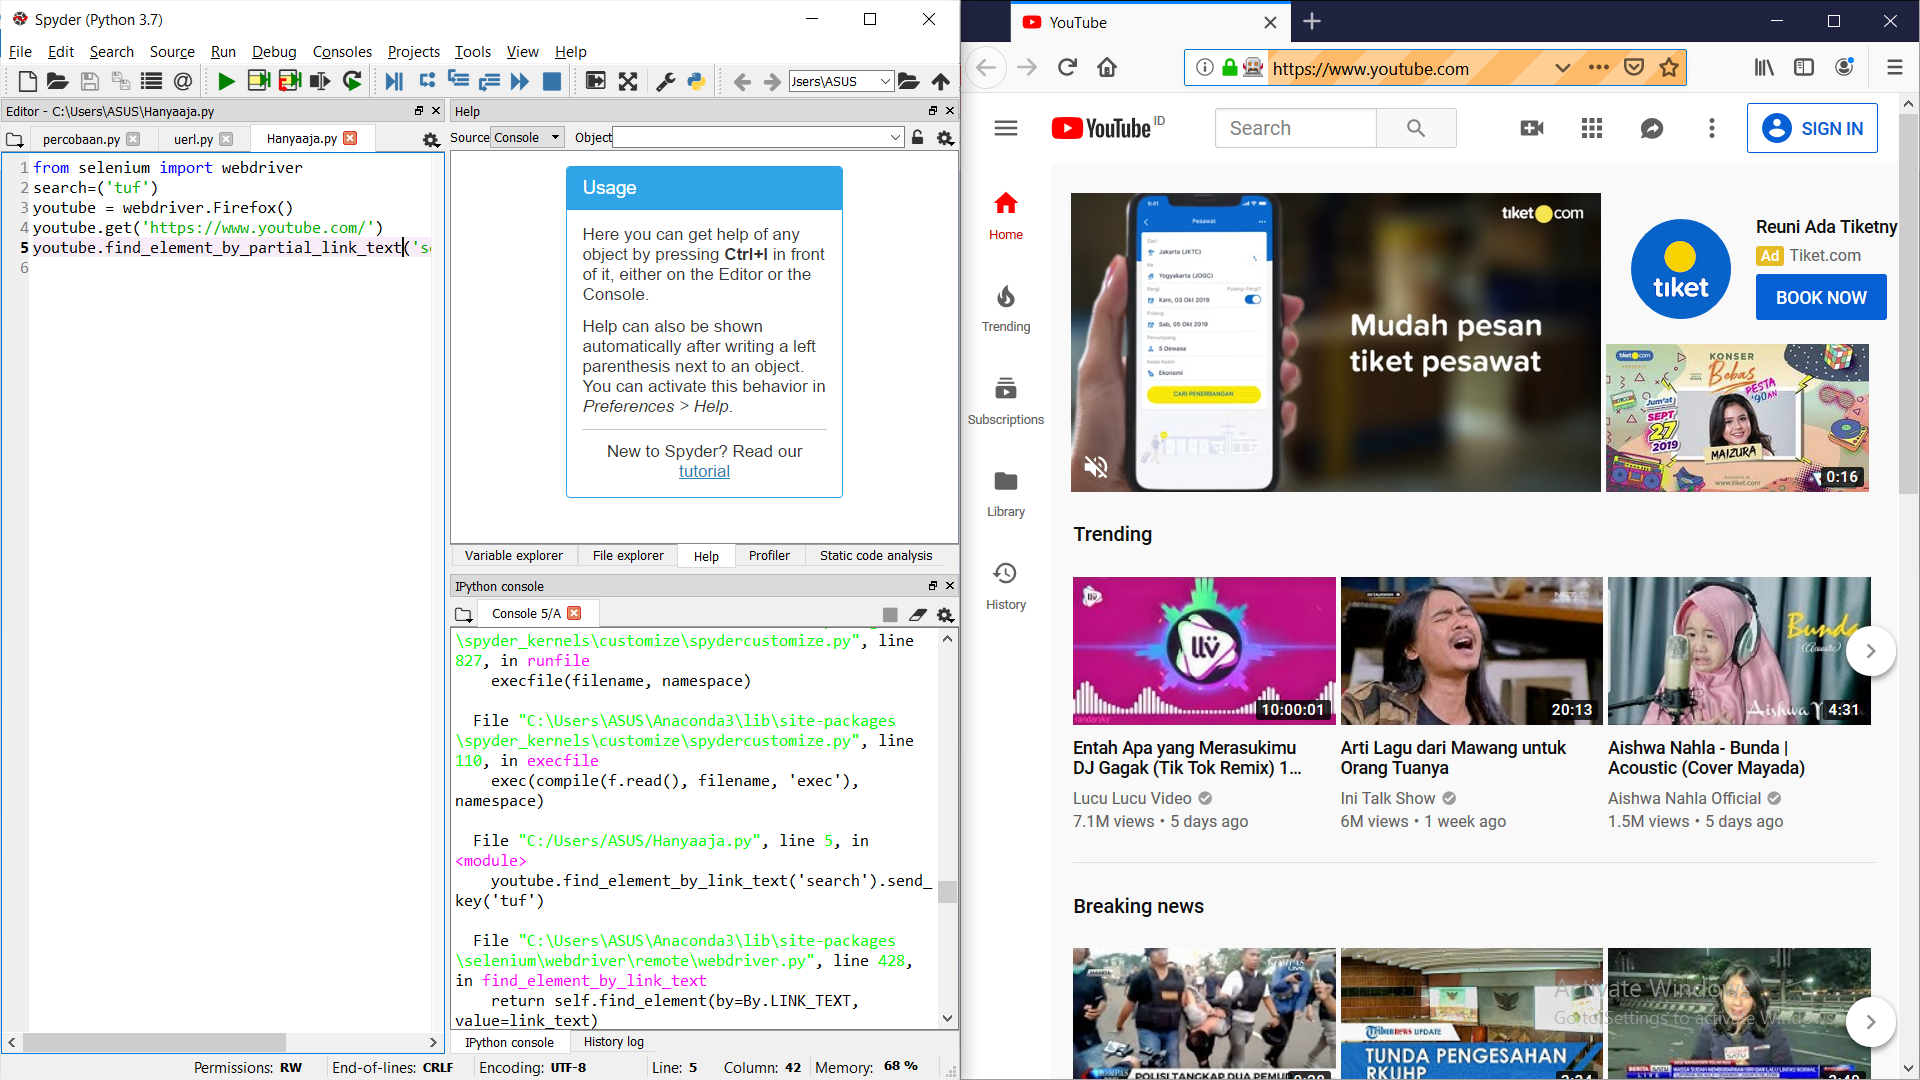
\includegraphics[scale=0.3]{figure/hasilTes/6.png}
    \label{gambar 1}
\end{figure}

\vspace{3cm}

    \item Kita menggunakan find\_element\_by\_tag\_name sebagai Pemberikan text secara otomatis. Saat  Di run hasil pada menu search pada youtube tidak muncul text yang telah ditentukan. Dan pada Spyder {(unable to locate search element)}
\begin{figure}[!htbp]
    \centering
    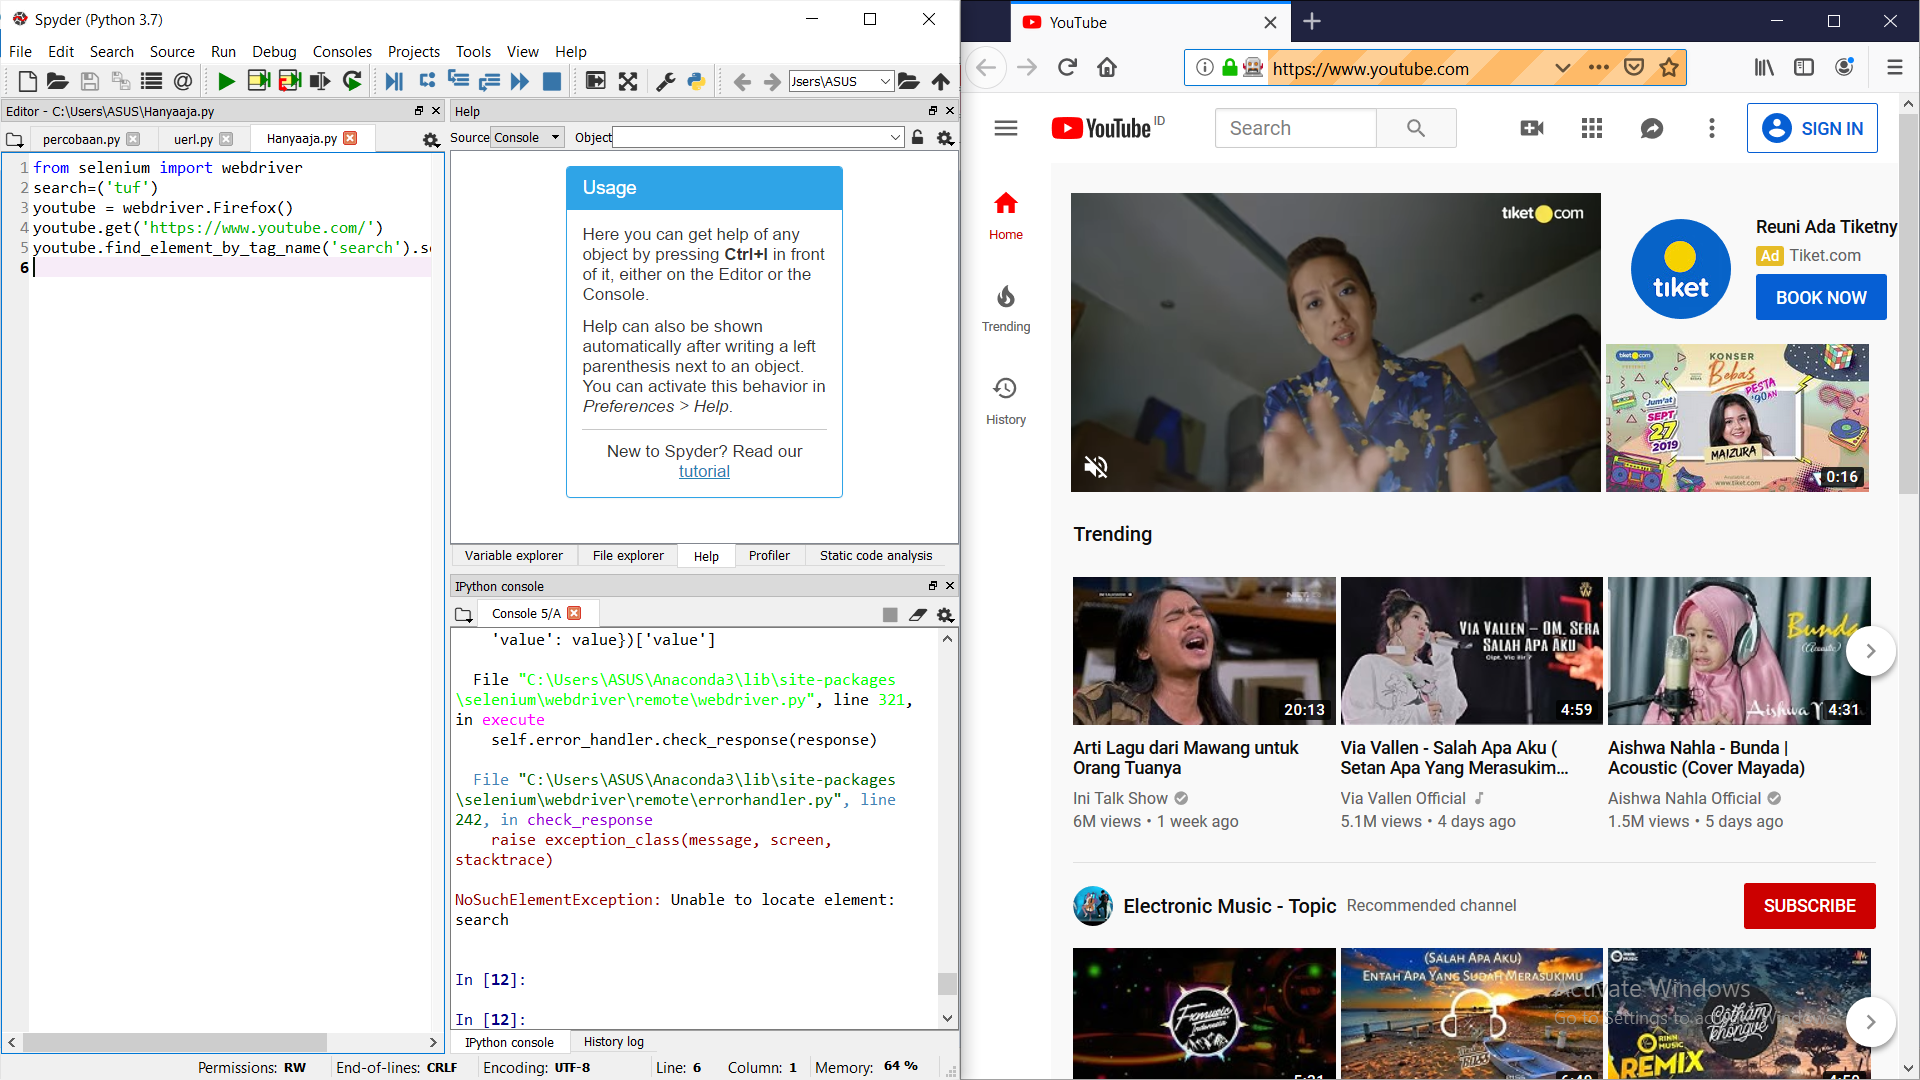
\includegraphics[scale=0.3]{figure/hasilTes/7.png}
    \label{gambar 1}
\end{figure}

\vspace{6cm}
    
    \item Kita menggunakan find\_element\_by\_xpath sebagai Pemberikan text secara otomatis. Saat  Di run hasil pada menu search pada youtube tidak muncul text yang telah ditentukan. Dan pada Spyder {(unable to locate search element)}
\begin{figure}[!htbp]
    \centering
    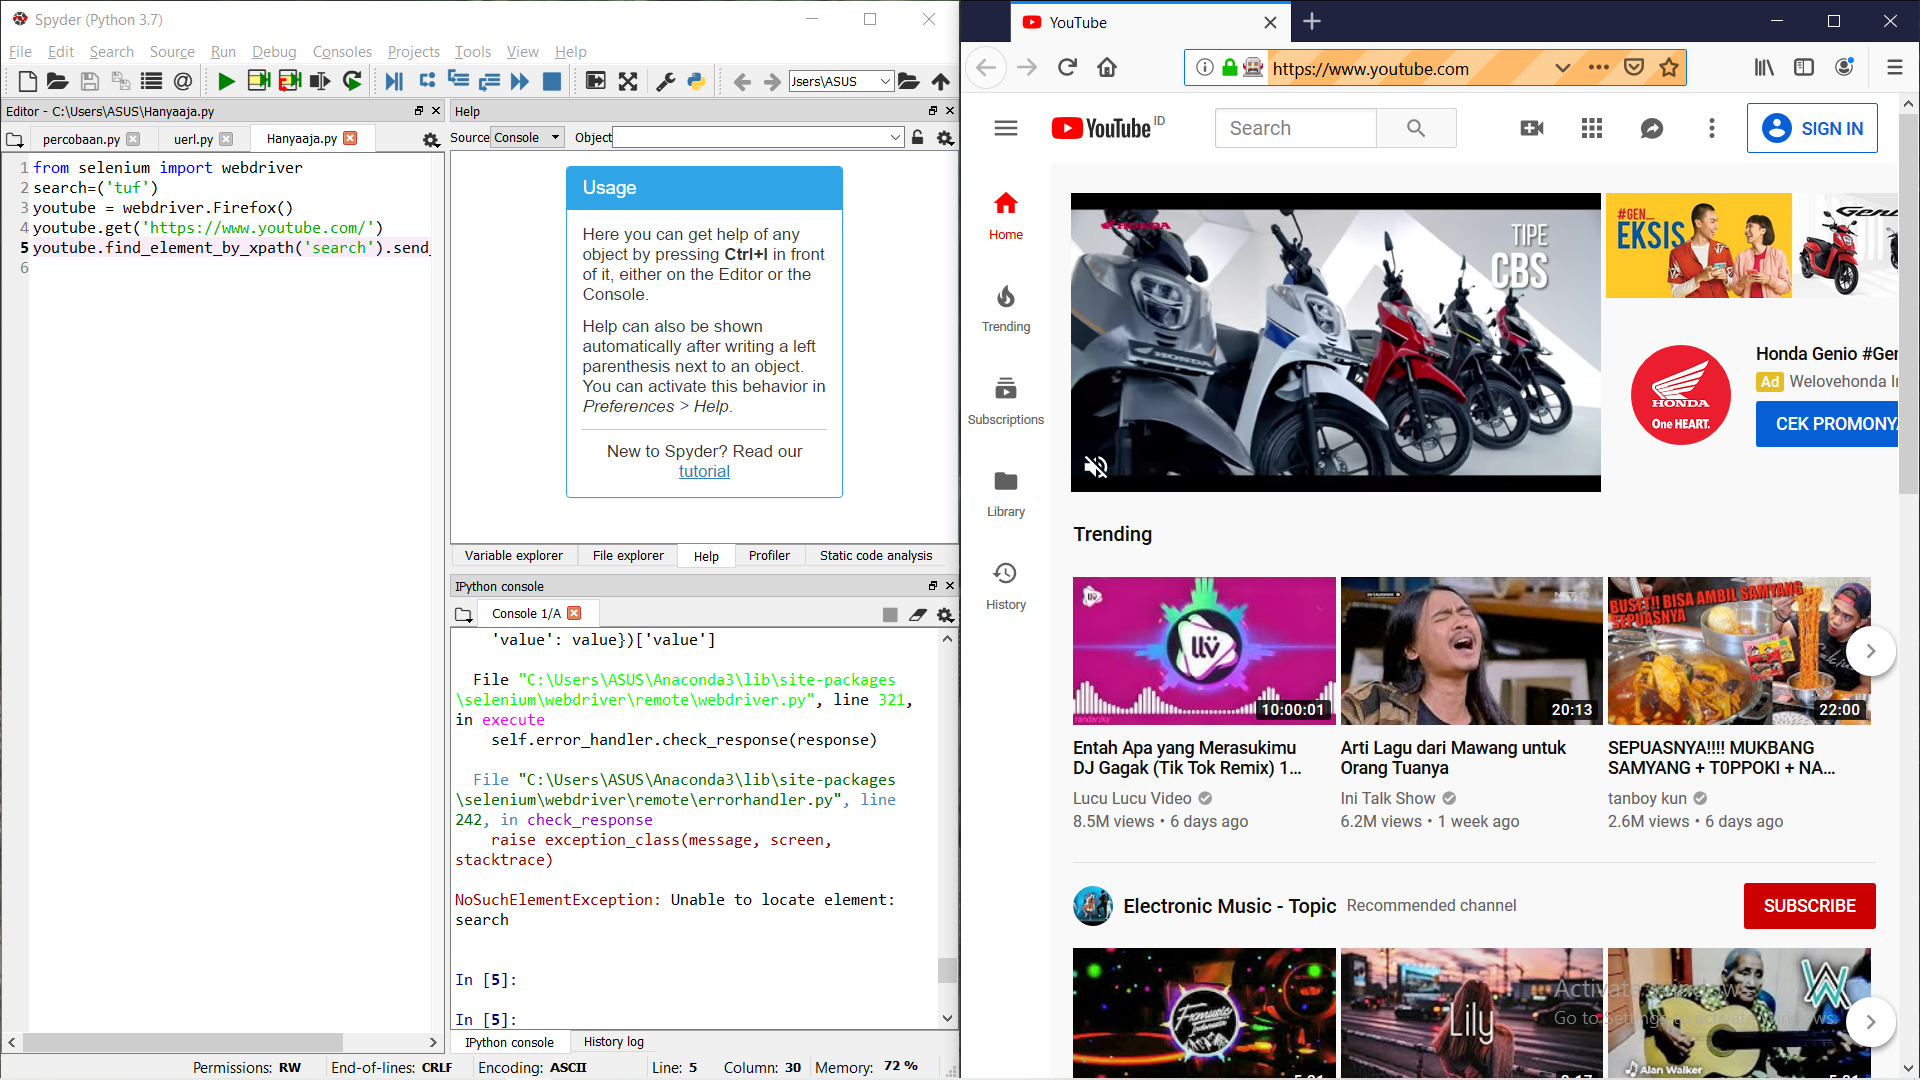
\includegraphics[scale=0.3]{figure/hasilTes/8.png}
    \label{gambar 1}
\end{figure}

    \item Kita menggunakan find\_elements sebagai Pemberikan text secara otomatis. Saat  Di run hasil pada menu search pada youtube tidak muncul text yang telah ditentukan. Dan pada Spyder {(unknown variant 'search')}
\begin{figure}[!htbp]
    \centering
    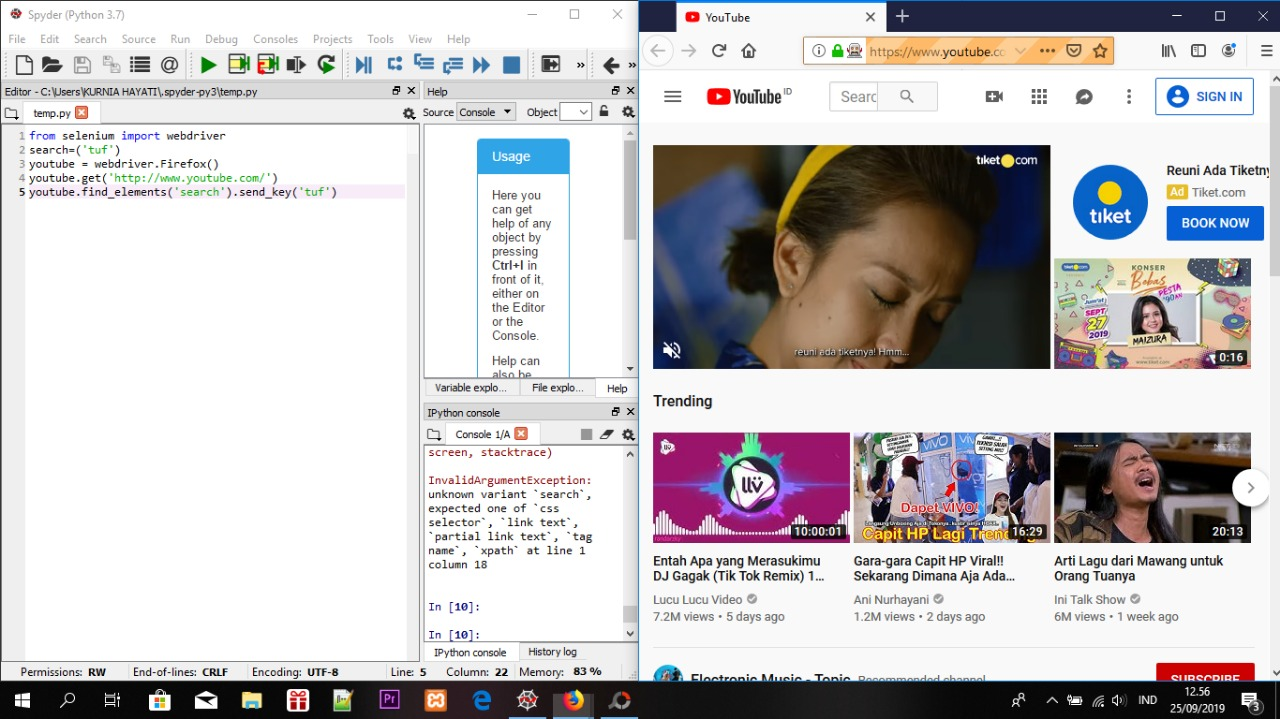
\includegraphics[scale=0.3]{figure/hasilTes/9.jpg}
    \label{gambar 1}
\end{figure}

    \item Kita menggunakan find\_elements\_by\_css\_selector sebagai Pemberikan text secara otomatis. Saat  Di run hasil pada menu search pada youtube tidak muncul text yang telah ditentukan. Dan pada Spyder {(list object has not attribut send\_key)}
\begin{figure}[!htbp]
    \centering
    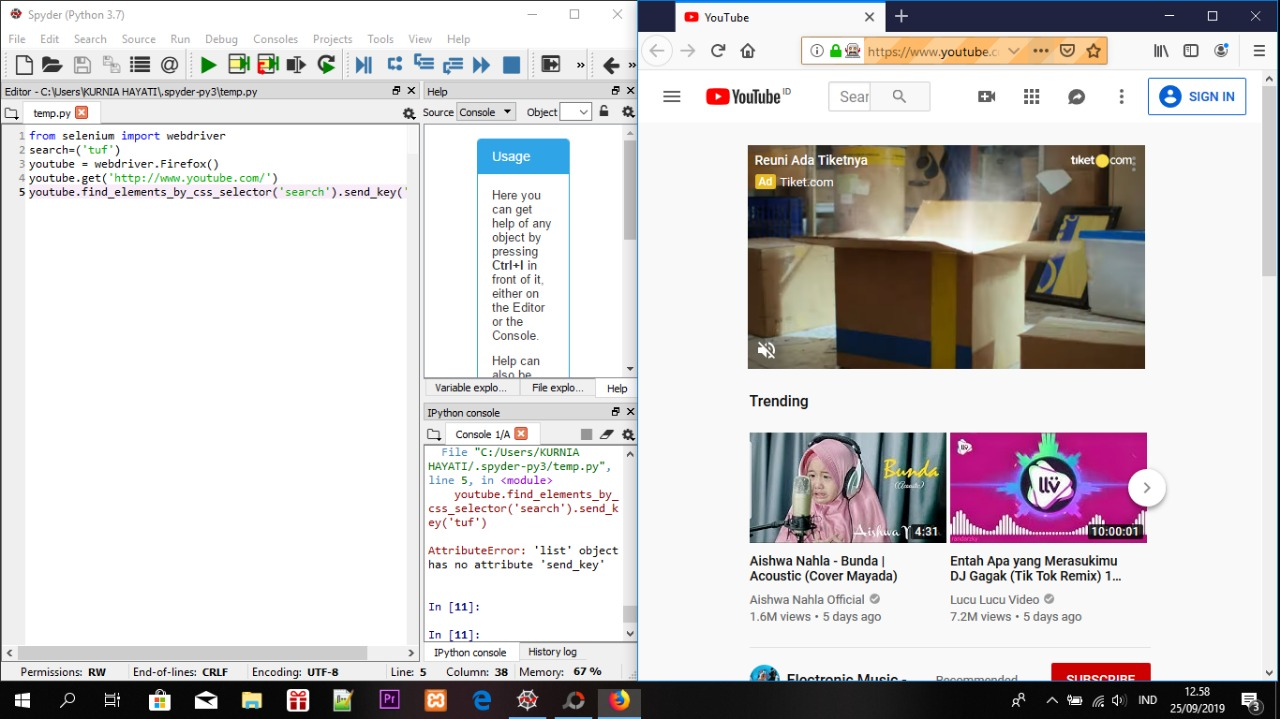
\includegraphics[scale=0.3]{figure/hasilTes/10.jpeg}
    \label{gambar 1}
\end{figure}

    \item Kita menggunakan find\_elements\_by\_name sebagai Pemberikan text secara otomatis. Saat  Di run hasil pada menu search pada youtube tidak muncul text yang telah ditentukan. Dan pada Spyder {(unable to locate search element)}
\begin{figure}[!htbp]
    \centering
    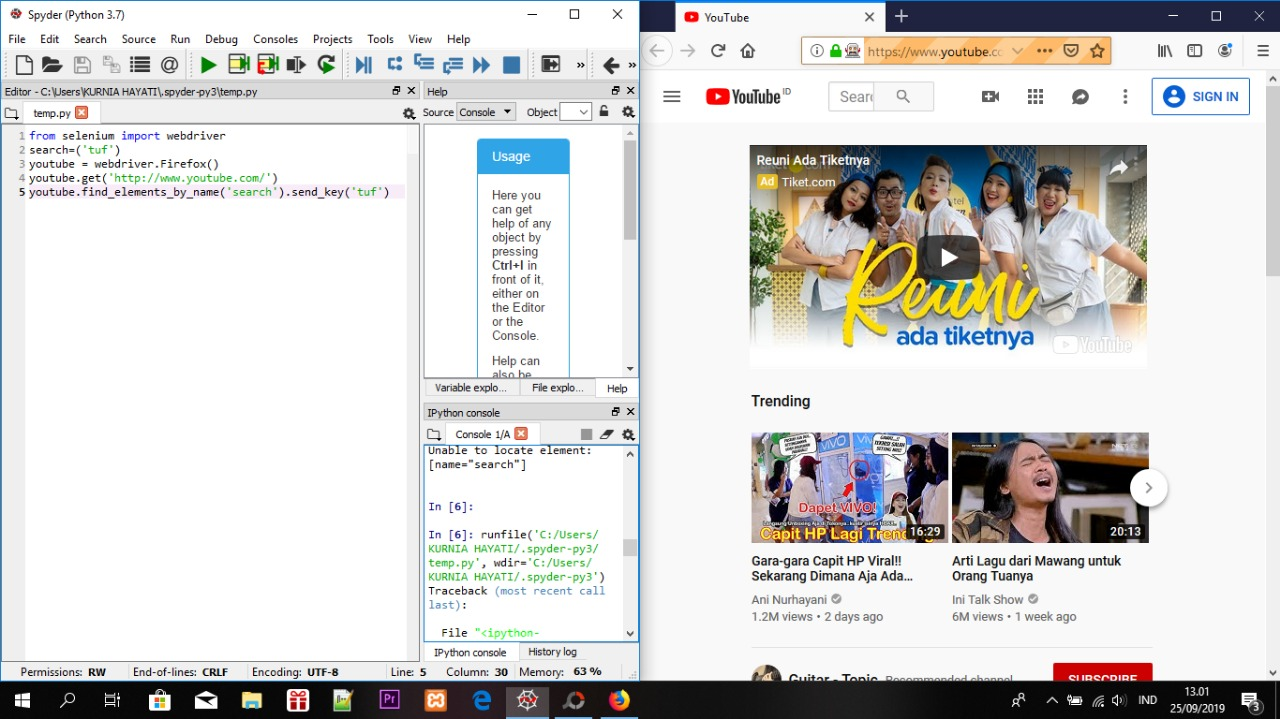
\includegraphics[scale=0.3]{figure/hasilTes/11.jpeg}
    \label{gambar 1}
\end{figure}

    \item Kita menggunakan find\_elements\_by\_partial\_link\_text sebagai Pemberikan text secara otomatis. Saat  Di run hasil pada menu search pada youtube tidak muncul text yang telah ditentukan. Dan pada Spyder {(unable to locate search element)}
\begin{figure}[!htbp]
    \centering
    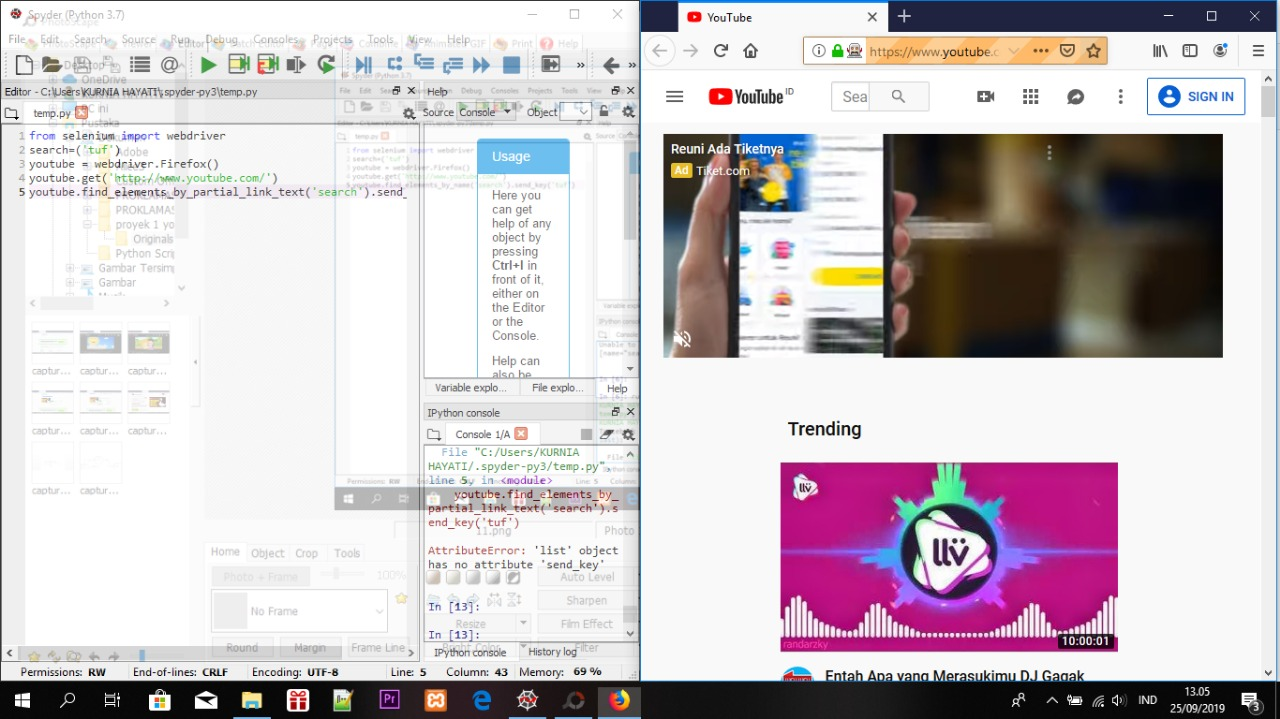
\includegraphics[scale=0.3]{figure/hasilTes/12.jpeg}
    \label{gambar 1}
\end{figure}

\vspace{1cm}

    \item Kita menggunakan find\_elements\_by\_tag\_name sebagai Pemberikan text secara otomatis. Saat  Di run hasil pada menu search pada youtube tidak muncul text yang telah ditentukan. Dan pada Spyder {(list object has not attribut send\_key)}
\begin{figure}[!htbp]
    \centering
    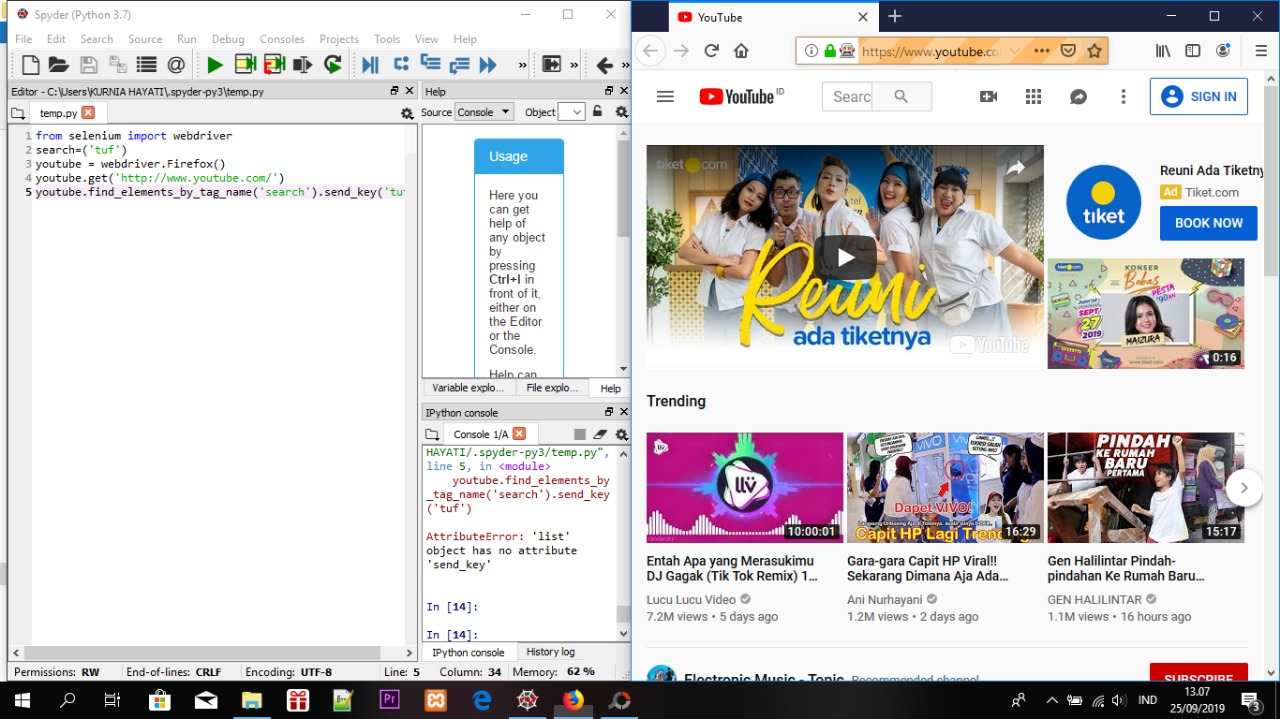
\includegraphics[scale=0.3]{figure/hasilTes/13.jpeg}
    \label{gambar 1}
\end{figure}

    \item Kita menggunakan find\_elements\_by xpath sebagai Pemberikan text secara otomatis. Saat  Di run hasil pada menu search pada youtube tidak muncul text yang telah ditentukan. Dan pada Spyder {(list object has not attribut send\_key)}
\begin{figure}[!htbp]
    \centering
    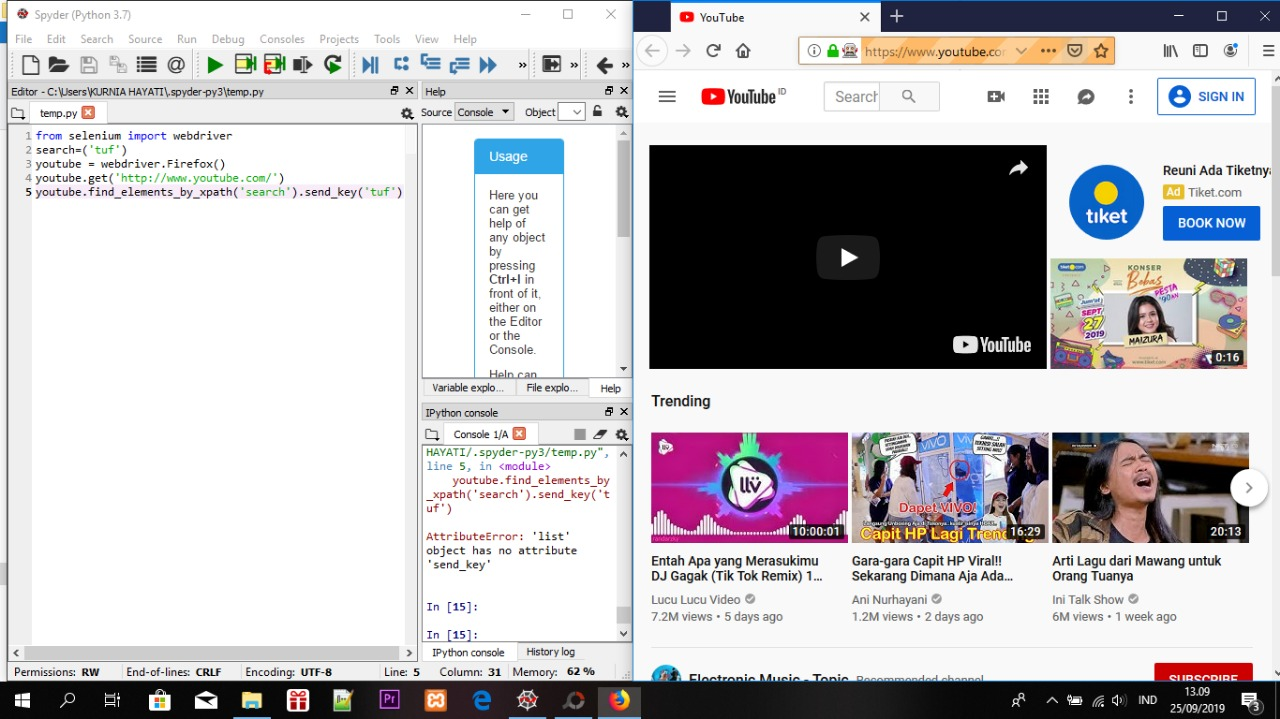
\includegraphics[scale=0.3]{figure/hasilTes/14.jpeg}
    \label{gambar 1}
\end{figure}
\end{enumerate}

\subsection{Hasil Pengujian}
Hasil dari uji diatas dengan berberapa cara tidak berhasil dalam memberikan text pada menu pencarian pada youtube sehingga pada code program selenium spyder (Anaconda 3) diubah dapat diliahat sebagi berikut:

\begin{figure}[!htbp]
    \centering
    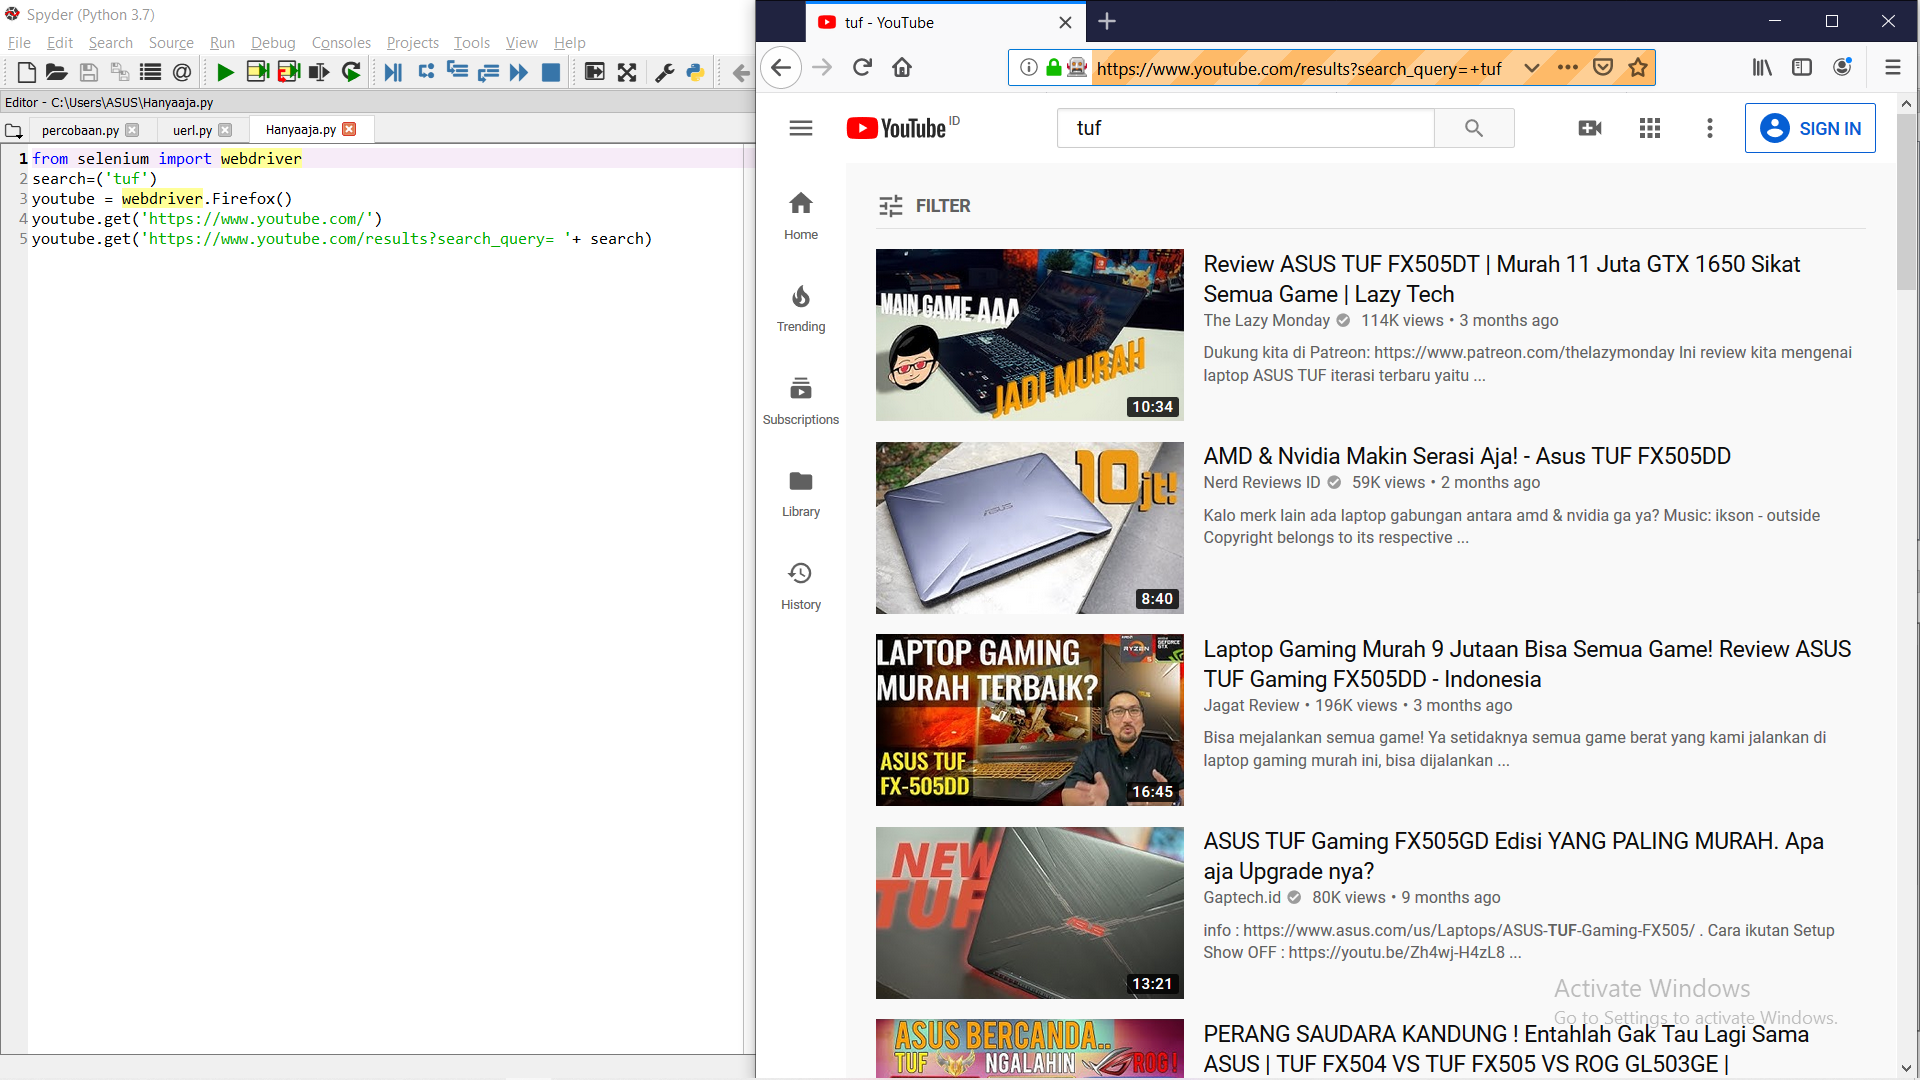
\includegraphics[scale=0.3]{figure/akhirnya.png}
    \label{gambar 1}
\end{figure}

\begin{enumerate}
    \item Dimana ditambahkan variable search dimana berfungsi sebagi media pencarian judul video yang akan dicari.
    \item Kemudia pada youtube.get('https://www.youtube.com/results?search\_query= '+ search)
    Ditambahkan dengan simbol + dengan variable search telah dibuat.
\end{enumerate}
